\chapter{Hệ có ràng buộc và chuyển động Hamilton}

\lectureoverview{Hai hệ có ràng buộc cho thấy vì sao cơ học Lagrange hiệu quả đến vậy: một khi đã chọn được các tọa độ thích hợp, các phương trình chuyển động và các định luật bảo toàn của chúng suy ra mà không cần tính tường minh các lực ràng buộc. Chính những ví dụ ấy sau đó dẫn tới cơ học Hamilton, trong đó các tọa độ và xung lượng tạo thành không gian pha, dao động tử điều hòa trở thành một phép quay cứng, và hai phương trình bậc nhất của Hamilton thay thế từng phương trình Euler--Lagrange bậc hai.}

\section{Giải một bài toán cơ học nghĩa là gì}

Mục đích trước mắt của phương pháp Lagrange là rất thực dụng. Một cái nêm trượt trên sàn và một con lắc kép đều có thể được xử lý bằng các định luật Newton, nhưng các lực tiếp xúc và lực căng chưa biết nhanh chóng khiến việc theo dõi các đại lượng trở nên rắc rối. Một khi đã biết các quy tắc của cơ học Lagrange, cùng những bài toán ấy trở thành một chuỗi bước được kiểm soát:
\begin{enumerate}
  \item chọn các tọa độ độc lập gắn nhãn một cấu hình tức thời;
  \item biểu diễn động năng và thế năng theo các tọa độ ấy;
  \item lập \(L=T-V\) và áp dụng các phương trình Euler--Lagrange.
\end{enumerate}

Với mục đích hiện tại, một bài toán đã được coi là \emph{đã giải xong} ngay khi các phương trình chuyển động của nó được viết xuống một cách đúng đắn. Ta vẫn có thể muốn một quỹ đạo dưới dạng giải tích tường minh, nhưng đó là một câu hỏi riêng. Các phương trình vi phân phi tuyến có thể được tích phân số một khi thiết lập cơ học đã hoàn tất. Phần khó thường không phải là phép tích phân; mà là tìm ra các biến đưa các ràng buộc vào mà không đưa thêm những lực chưa biết dư thừa.

\section{Một hạt trượt trên một cái nêm đang chuyển động}

Xét một cái nêm khối lượng \(M\) bị ràng buộc chỉ được trượt không ma sát dọc theo một mặt phẳng ngang. Một hạt điểm khối lượng \(m\) bị ràng buộc phải nằm trên mặt nghiêng. Có hai bậc tự do: một bậc cho biết cái nêm ở đâu, và một bậc cho biết hạt ở đâu trên cái nêm.

Đặt
\begin{equation}
  \begin{aligned}
    X&=\text{horizontal position of the wedge corner},\\
    x&=\text{horizontal displacement of the particle}\\[-0.2em]
     &\phantom{={}}\text{from that corner}.
  \end{aligned}
  \label{eq:l6-wedge-coordinates}
\end{equation}
Tọa độ ngang tuyệt đối của hạt vì thế là \(X+x\). Cách chọn này không duy nhất. Thay vào đó, ta cũng có thể dùng khoảng cách dọc theo mặt dốc hoặc tọa độ ngang tuyệt đối của hạt. Bất kỳ cặp không dư thừa nào gắn nhãn cùng các cấu hình đều hợp lệ, dù một số cặp làm lộ rõ cấu trúc hơn những cặp khác.

Với góc dốc cố định \(\beta\), độ dời thẳng đứng \(y\) không phải là một tọa độ độc lập:
\begin{equation}
  y=x\tan\beta,
  \qquad
  \dot y=\dot x\tan\beta.
  \label{eq:l6-wedge-constraint}
\end{equation}
Ta chuyên biệt tới \(\beta=45^\circ\), sao cho \(y=x\) và
\(\dot y=\dot x\). Sự đơn giản hóa này loại bỏ các hệ số lượng giác mà không làm thay đổi ý nghĩa của ví dụ.

\begin{figure}[htbp]
  \centering
  \includegraphics[width=0.84\textwidth]{lecture_06_figure_06.png}
  \caption{Cái nêm chuyển động, hạt bị ràng buộc, và các thành phần vận tốc theo phương ngang và phương thẳng đứng dùng trong ví dụ \(45^\circ\).}
  \lectureframe{00:10:25}
\end{figure}

Cái nêm có động năng
\begin{equation}
  T_{M}=\frac{M}{2}\dot X^2.
  \label{eq:l6-wedge-kinetic}
\end{equation}
Vận tốc ngang tuyệt đối của hạt là \(\dot X+\dot x\), còn vận tốc thẳng đứng của nó là \(\dot x\). Do đó động năng của nó là
\begin{equation}
  T_m=\frac{m}{2}\left[(\dot X+\dot x)^2+\dot x^2\right].
  \label{eq:l6-particle-kinetic}
\end{equation}
Lấy mốc không của thế năng hấp dẫn tại \(x=0\), ta có \(V=mgx\).
Vì vậy
\begin{equation}
  L=\frac{M}{2}\dot X^2
    +\frac{m}{2}\left[(\dot X+\dot x)^2+\dot x^2\right]
    -mgx.
  \label{eq:l6-wedge-lagrangian}
\end{equation}

\begin{figure}[htbp]
  \centering
  \includegraphics[width=0.86\textwidth]{lecture_06_figure_07.png}
  \caption{Hình học của cái nêm, \(V=mgx\), và hai phần đóng góp của động năng được ghép lại trên bảng.}
  \lectureframe{00:14:15}
\end{figure}

\subsection{Xung lượng chính tắc được định nghĩa bởi Lagrangian}

Các xung lượng chính tắc được định nghĩa bởi Lagrangian, chứ không phải bằng một phỏng đoán dựa trên vận tốc của một hạt đơn lẻ:
\begin{align}
  p_X&=\frac{\partial L}{\partial\dot X}
      =M\dot X+m(\dot X+\dot x),
      \label{eq:l6-wedge-pX}\\
  p_x&=\frac{\partial L}{\partial\dot x}
      =m(\dot X+\dot x)+m\dot x.
      \label{eq:l6-wedge-px}
\end{align}
Biểu thức thứ nhất là tổng động lượng theo phương ngang thông thường: cái nêm đóng góp \(M\dot X\), và hạt đóng góp \(m(\dot X+\dot x)\). Ở đây nó xuất hiện như xung lượng liên hợp với tọa độ \(X\).

\begin{figure}[htbp]
  \centering
  \includegraphics[width=0.86\textwidth]{lecture_06_figure_08.png}
  \caption{Các xung lượng chính tắc liên hợp với tọa độ của cái nêm \(X\) và tọa độ tương đối của hạt \(x\).}
  \lectureframe{00:18:05}
\end{figure}

Lagrangian không phụ thuộc tường minh vào \(X\). Một phép tịnh tiến theo phương ngang của toàn bộ hệ tác dụng như
\begin{equation}
  \delta X=\epsilon,
  \qquad
  \delta x=0.
  \label{eq:l6-wedge-translation}
\end{equation}
Quy tắc đối xứng vô cùng bé tổng quát
\begin{equation}
  \delta q_i=\epsilon f_i(q),
  \qquad
  Q=\sum_i p_i f_i
  \label{eq:l6-noether-rule}
\end{equation}
vì thế cho \(Q=p_X\). Tương đương, \(X\) là tọa độ chu kỳ và
\begin{equation}
  \dot p_X=\frac{\partial L}{\partial X}=0.
  \label{eq:l6-wedge-conservation}
\end{equation}

Không có đối xứng tịnh tiến thẳng đứng tương ứng. Cái nêm không được phép chuyển động theo phương thẳng đứng, và việc thay đổi độ cao của hạt làm thay đổi thế năng hấp dẫn. Động lượng ngang được bảo toàn; động lượng thẳng đứng của phân hệ có ràng buộc này thì không.

Đối với tọa độ tương đối, phương trình Euler--Lagrange là
\begin{equation}
  \dot p_x=\frac{\partial L}{\partial x}=-mg.
  \label{eq:l6-wedge-force}
\end{equation}
Dòng này đã cần sửa dấu trên bảng. Cách chắc chắn là bắt đầu từ \(L=T-V\): vì \(V=mgx\), đạo hàm của Lagrangian là \(-mg\). Việc \(x\) được đưa vào như một độ dời ngang không loại bỏ trọng lực khỏi phương trình của nó, vì ràng buộc gắn độ dời ngang ấy với độ cao thẳng đứng \(y=x\).

Không có lực pháp tuyến hay phản lực nào xuất hiện. Những lực như vậy sẽ nhận bất kỳ giá trị nào cần thiết để duy trì các ràng buộc. Phương pháp Newton sẽ đưa chúng vào và giải chúng cùng với các gia tốc; các tọa độ suy rộng đã làm cho chúng trở nên không cần thiết.

\section{Con lắc kép và nghệ thuật chọn tọa độ}

Bây giờ treo hai khối lượng đơn vị bằng hai thanh không khối lượng, mỗi thanh dài đơn vị. Thanh thứ nhất hợp với phương thẳng đứng hướng xuống một góc \(\theta\). Đối với bậc tự do thứ hai, ta có một lựa chọn. Ta có thể dùng một góc tuyệt đối thứ hai \(\phi\), hoặc dùng góc tương đối \(\alpha\) giữa hai thanh.

Góc tương đối là lựa chọn bộc lộ nhiều điều hơn. Tạm thời bỏ qua trọng lực. Một phép quay cứng của toàn bộ hệ làm thay đổi phương tuyệt đối nhưng không làm thay đổi góc giữa hai thanh:
\begin{equation}
  \theta\longrightarrow\theta+\epsilon,
  \qquad
  \alpha\longrightarrow\alpha.
  \label{eq:l6-double-rotation}
\end{equation}
Với cách chọn này, đối xứng quay chỉ tác động lên một tọa độ. Điều đó không làm cho các hệ tọa độ khác trở nên sai. Nó làm cho đối xứng, và do đó đại lượng bảo toàn, dễ thấy hơn.

\begin{figure}[htbp]
  \centering
  \includegraphics[width=0.76\textwidth]{lecture_06_figure_09.png}
  \caption{Con lắc kép với \(\theta\) là góc tuyệt đối thứ nhất và \(\alpha\) là góc của thanh thứ hai tương đối so với thanh thứ nhất.}
  \lectureframe{00:29:20}
\end{figure}

Để thu được động năng, hãy dùng các tọa độ Đề-các như những công cụ ghi sổ tạm thời. Với tọa độ thẳng đứng được đo theo chiều đi xuống, quả nặng thứ nhất ở
\begin{equation}
  x_1=\sin\theta,
  \qquad
  y_1=\cos\theta,
  \label{eq:l6-bob-one-position}
\end{equation}
và do đó
\begin{equation}
  \dot x_1=\dot\theta\cos\theta,
  \qquad
  \dot y_1=-\dot\theta\sin\theta,
  \qquad
  \dot x_1^2+\dot y_1^2=\dot\theta^2.
  \label{eq:l6-bob-one-velocity}
\end{equation}
Quả nặng thứ hai ở
\begin{align}
  x_2&=\sin\theta+\sin(\theta+\alpha),\\
  y_2&=\cos\theta+\cos(\theta+\alpha),
  \label{eq:l6-bob-two-position}
\end{align}
nên, chẳng hạn,
\begin{equation}
  \dot x_2=\dot\theta\cos\theta
  +(\dot\theta+\dot\alpha)\cos(\theta+\alpha),
  \label{eq:l6-bob-two-xvelocity}
\end{equation}
với một biểu thức tương tự cho \(\dot y_2\).

\begin{figure}[htbp]
  \centering
  \includegraphics[width=0.88\textwidth]{lecture_06_figure_10.png}
  \caption{Các tọa độ Đề-các phụ trợ cho hai quả nặng. Chúng được dùng để tính các vận tốc, chứ không được đưa vào như các bậc tự do bổ sung.}
  \lectureframe{00:35:25}
\end{figure}

Cộng hai động năng lại cho ta kết quả nhất quán dưới đây. Hạng chéo xuất phát từ
\begin{equation*}
  \cos A\cos B+\sin A\sin B=\cos(A-B).
\end{equation*}
\begin{equation}
  T=\dot\theta^2
    +\frac12(\dot\theta+\dot\alpha)^2
    +\dot\theta(\dot\theta+\dot\alpha)\cos\alpha.
  \label{eq:l6-double-kinetic}
\end{equation}

\begin{classroomqa}
  \audiencequestion{Biểu thức này đã bao gồm động năng của cả hai quả nặng chưa, và có bị mất hệ số một phần hai không?
  \lecturetimestamp{00:38:06--00:38:27}}
  \lecturerresponse{Nó bao gồm cả hai. Nó xuất phát từ
  \(\tfrac12(\dot x_1^2+\dot y_1^2+\dot x_2^2+\dot y_2^2)\).
  Hai phần đóng góp bằng nhau gộp lại tạo ra hạng đầu tiên
  \(\dot\theta^2\); không thiếu hệ số nào.}
\end{classroomqa}

Không có trọng lực, \(L=T\) không chứa \(\theta\) một cách tường minh. Do đó
\begin{equation}
  \dot p_\theta=\frac{\partial L}{\partial\theta}=0,
  \label{eq:l6-double-angular-conservation}
\end{equation}
và \(p_\theta\) là tổng xung lượng góc. Hãy lưu ý ý nghĩa chính xác của phát biểu rằng \(\theta\) không xuất hiện: \(\dot\theta\) dĩ nhiên có xuất hiện, nhưng bản thân tọa độ chưa lấy đạo hàm thì không.

Khôi phục trọng lực phá vỡ đối xứng quay toàn cục. Với quy ước phương thẳng đứng hướng xuống ở trên, một cách chọn mốc không thuận tiện cho ta
\begin{equation}
  V=-g(y_1+y_2)
   =-g\left[2\cos\theta+\cos(\theta+\alpha)\right].
  \label{eq:l6-double-potential}
\end{equation}
Thêm một hằng số sẽ không làm thay đổi điều gì. Điểm quan trọng là \(\theta\) nay xuất hiện tường minh, nên xung lượng liên hợp với nó không còn được bảo toàn. Năng lượng vẫn được bảo toàn vì Lagrangian không phụ thuộc tường minh vào thời gian.

\begin{classroomqa}
  \audiencequestion{Có phải \(\dot\theta-\dot\alpha\) trên bảng phải là
  \(\dot\theta+\dot\alpha\) không?
  \lecturetimestamp{00:43:00--00:43:54}}
  \lecturerresponse{Cách định hướng được dùng ở đây đòi hỏi dấu cộng. Đó là quy ước trong Eq.~\eqref{eq:l6-bob-two-position} và được duy trì xuyên suốt trong động năng ở Eq.~\eqref{eq:l6-double-kinetic}. Nếu đảo ngược định nghĩa chiều dương của \(\alpha\) thì các dấu tương ứng sẽ đổi, nhưng khi đó mọi chỗ xuất hiện đều phải được đổi một cách nhất quán. Trên bảng đã trộn lẫn hai quy ước ấy.}
\end{classroomqa}

\begin{figure}[htbp]
  \centering
  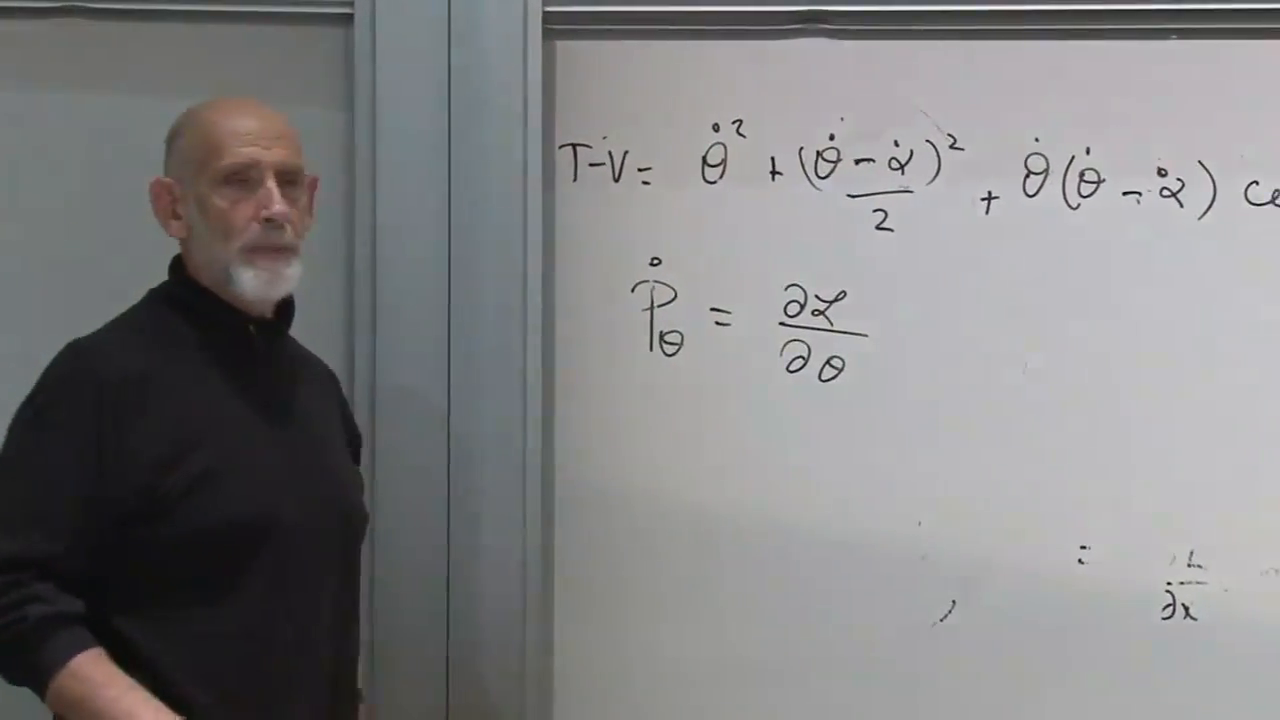
\includegraphics[width=0.84\textwidth]{lecture_06_figure_02.png}
  \caption{Phép tính con lắc khi không có trọng lực và
  \(\dot p_\theta=\partial L/\partial\theta\). Dòng trên của bảng giữ nguyên ký hiệu cục bộ không nhất quán về dấu được bàn trong câu hỏi; công thức đã chuẩn hóa là Eq.~\eqref{eq:l6-double-kinetic}.}
  \lectureframe{00:45:50}
\end{figure}

Khi đã biết \(T\) và \(V\), các phương trình còn lại thu được bằng phép lấy đạo hàm. Lực căng của các thanh và các lực áp đặt độ dài cố định lại một lần nữa biến mất vào cách chọn tọa độ.

\subsection{Bảo toàn hàm ý điều gì và không hàm ý điều gì}

\begin{classroomqa}
  \audiencequestion{Có thể nhìn trực tiếp từ các phương trình để biết con lắc kép có hỗn loạn hay không không?
  \lecturetimestamp{00:44:57--00:45:25}}
  \lecturerresponse{Thường là không, nếu chỉ quan sát đơn giản. Khi các tham số hoặc các năng lượng thay đổi, một hệ có thể chuyển từ hành vi đều đặn sang hành vi hỗn loạn. Chủ đề này đòi hỏi nhiều cấu trúc hơn là diện mạo thô của các phương trình, và sẽ được bàn sau.}
\end{classroomqa}

\begin{classroomqa}
  \audiencequestion{Trong một hệ bảo toàn, có phải mọi \(\dot p_i\) đều bằng không không?
  \lecturetimestamp{00:45:25--00:46:24}}
  \lecturerresponse{Không. Phương trình tổng quát là
  \(\dot p_i=\partial L/\partial q_i\). Nó chỉ triệt tiêu khi \(q_i\) là tọa độ chu kỳ. Tọa độ chu kỳ là trường hợp đặc biệt đơn giản trong đó một đối xứng đã được viết dưới dạng dịch chuyển một tọa độ trong khi giữ cố định các tọa độ khác.}
\end{classroomqa}

Nếu mục tiêu duy nhất là tiến hóa số, một hệ tọa độ bất tiện vẫn dùng được; nó chỉ tạo ra các phương trình dài hơn. Phần thưởng của một hệ khéo chọn mang tính khái niệm: xung lượng bảo toàn hiện rõ trước khi các phương trình được giải.

\begin{classroomqa}
  \audiencequestion{Không có trọng lực, con lắc kép có hành xử đơn giản như một con lắc tự do đơn không?
  \lecturetimestamp{00:47:02--00:47:35}}
  \lecturerresponse{Một rotor tự do đơn quay đều vì xung lượng góc duy nhất của nó xác định chuyển động của nó. Một con lắc kép có thể thực hiện chuyển động tương đối rất phức tạp trong khi vẫn bảo toàn tổng xung lượng góc. Nếu ban đầu cả hai vận tốc góc đều triệt tiêu thì nó đứng yên; nếu không, hai phần tương tác với nhau.}
\end{classroomqa}

\begin{classroomqa}
  \audiencequestion{Khi không có trọng lực, \(\dot\theta\) và \(\dot\alpha\) riêng rẽ có không đổi không?
  \lecturetimestamp{00:47:36--00:52:42}}
  \lecturerresponse{Không. Định luật bảo toàn nói \(\dot p_\theta=0\), chứ không phải \(\ddot\theta=0\) hoặc \(\ddot\alpha=0\). Biểu thức của \(p_\theta=\partial L/\partial\dot\theta\) chứa cả hai vận tốc góc và phụ thuộc vào \(\alpha\). Các thanh truyền mômen xoắn, cho phép hai quả nặng trao đổi xung lượng góc và năng lượng. Điều này tương tự như hai khối lượng nối với nhau bằng một lò xo: tổng động lượng và vận tốc khối tâm là không đổi, còn các vận tốc riêng lẻ thì dao động. Đối tượng tương tự trong chuyển động quay là một tổ hợp tập thể xác định, chứ không phải riêng từng góc.}
\end{classroomqa}

\begin{classroomqa}
  \audiencequestion{Các lực làm trao đổi xung lượng góc có được truyền qua các thanh không?
  \lecturetimestamp{00:52:43--00:53:34}}
  \lecturerresponse{Có. Một lực được truyền dọc theo một thanh không nhất thiết đi qua chốt quay của chuyển động kia, nên nó có thể gây ra mômen xoắn. Mômen xoắn đơn giản là xu hướng gây quay của một lực, và ở đây nó tạo ra các gia tốc góc riêng lẻ khác không.}
\end{classroomqa}

\section{Hamiltonian như một hình thức mô tả thứ ba}

Hamiltonian là năng lượng, nhưng đó mới chỉ là ý nghĩa thứ nhất của nó. Nó cũng là nền tảng của một hình thức mô tả thứ ba của cơ học. Các phương trình Newton dùng lực và gia tốc. Nguyên lý tác dụng dừng cho các phương trình Euler--Lagrange. Cơ học Hamilton tương đương với mô tả Lagrange đối với các hệ chính quy, nhưng các biến và hình học của nó có diện mạo khác.

Thay vì \(q_i\) và \(\dot q_i\), hãy dùng \(q_i\) và các xung lượng liên hợp của chúng
\(p_i\).  Trạng thái của một hệ có \(n\) bậc tự do cần \(2n\)
số trong cả hai cách mô tả: vị trí và vận tốc, hoặc vị trí và
xung lượng.  Cầu nối giữa chúng là
\begin{equation}
  p_i=\frac{\partial L}{\partial\dot q_i}.
  \label{eq:l6-legendre-map}
\end{equation}
Khi có thể giải ngược các hệ thức này để được các vận tốc
\(\dot q_i(q,p)\), ta định nghĩa
\begin{equation}
  H(q,p)=\sum_i p_i\dot q_i-L(q,\dot q).
  \label{eq:l6-hamiltonian-definition}
\end{equation}
Khi đó, các vận tốc ở vế phải được khử để biểu diễn theo \(q\) và \(p\).
Giả thiết khả nghịch này chính là giả thiết biến đổi Legendre chính quy.  Các
Lagrangian suy biến đòi hỏi lý thuyết ràng buộc tổng quát hơn; chúng không
được xử lý bằng phép dựng sơ cấp này.

\subsection{Tính khả nghịch trước giải tích}

Hãy nhớ lại một tập hữu hạn các trạng thái trừu tượng được nối với nhau bằng các mũi tên.  Một
quy tắc tất định vẫn có thể không khả nghịch nếu hai trạng thái trước đó cùng
đi tới một trạng thái về sau.  Tương lai là duy nhất, nhưng quá khứ thì không.  Đảo ngược
mọi mũi tên tạo ra khuyết điểm ngược lại: một trạng thái phân nhánh thành nhiều
tương lai.  Ở hình thứ nhất các mũi tên hội tụ; ở hình thứ hai chúng phân kỳ.

\begin{figure}[htbp]
  \centering
  \includegraphics[width=0.86\textwidth]{lecture_06_figure_11.png}
  \caption{Các ánh xạ trạng thái trừu tượng được dùng để đối chiếu các chu trình khả nghịch với
  sự hội tụ và phân kỳ bị cấm.}
  \lectureframe{00:56:20}
\end{figure}

Dòng Hamilton sẽ cung cấp phiên bản liên tục của phát biểu này.  Một
đám mây các điểm trong không gian pha có thể chuyển động và biến dạng, nhưng nó không thể hình thành một điểm hút
làm mất sự phân biệt giữa các trạng thái hoặc một nguồn tạo ra
nhiều tương lai từ một trạng thái.  Chứng minh sẽ được hoãn lại; hiện giờ,
các hình vẽ này gợi ra hình học.

\begin{classroomqa}
  \audiencequestion{Có nên hiểu sơ đồ trạng thái trừu tượng này như một
  vật chuyển động trong trường hấp dẫn không?
  \lecturetimestamp{00:58:02--00:58:35}}
  \lecturerresponse{Không.  Các chấm chỉ đơn thuần là các trạng thái trừu tượng và các mũi tên
  chỉ rõ một quy tắc thay đổi trạng thái.  Không có ý nghĩa không gian hay hấp dẫn nào
  được gán cho hình vẽ này.}
\end{classroomqa}

\begin{classroomqa}
  \audiencequestion{Làm thế nào để phân biệt một ánh xạ trạng thái hội tụ bị cấm
  với một hố đen?
  \lecturetimestamp{00:58:40--00:59:28}}
  \lecturerresponse{Chỉ với nhiều khó khăn và sự tinh tế.  Đó là một câu hỏi xác đáng,
  nhưng câu trả lời đúng đòi hỏi phải mô tả cẩn thận trạng thái đầy đủ và
  sự tiến hóa hấp dẫn lượng tử của nó.  Sơ đồ sơ cấp này không đủ
  để quyết định vấn đề ấy.}
\end{classroomqa}

\section{Một dao động tử thích nghi với không gian pha}

Trước khi suy ra các phương trình tổng quát, hãy xét một dao động tử điều hòa được viết
bằng các biến đã được thích nghi một cách có chủ ý:
\begin{equation}
  L=\frac{1}{2\omega}\dot q^2-\frac{\omega}{2}q^2.
  \label{eq:l6-rescaled-lagrangian}
\end{equation}
Xung lượng liên hợp của nó là
\begin{equation}
  p=\frac{\partial L}{\partial\dot q}=\frac{\dot q}{\omega},
  \qquad
  \dot q=\omega p.
  \label{eq:l6-rescaled-momentum}
\end{equation}
Thế vào phương trình ~\eqref{eq:l6-hamiltonian-definition} ta được
\begin{align}
  H&=p\dot q-L\\
   &=\omega p^2-\frac{\omega p^2}{2}+\frac{\omega q^2}{2}
    =\frac{\omega}{2}(p^2+q^2).
  \label{eq:l6-oscillator-hamiltonian}
\end{align}

\begin{figure}[htbp]
  \centering
  \includegraphics[width=0.86\textwidth]{lecture_06_figure_12.png}
  \caption{Biến đổi Legendre của dao động tử đã được thích nghi và Hamiltonian đối xứng
  \(H=\tfrac{\omega}{2}(p^2+q^2)\).}
  \lectureframe{01:08:20}
\end{figure}

Không gian của \(q\) và \(p\) là không gian pha.  Một bậc tự do cho một
mặt phẳng hai chiều; hai bậc tự do cho một không gian pha bốn chiều.  Ở năng lượng dao động tử cố định,
\begin{equation}
  p^2+q^2=\frac{2H}{\omega},
  \label{eq:l6-energy-circle}
\end{equation}
nên quỹ đạo nằm trên một đường tròn.  Bảo toàn năng lượng giới hạn chuyển động vào
một đường cong như vậy.

\begin{figure}[htbp]
  \centering
  \includegraphics[width=0.82\textwidth]{lecture_06_figure_13.png}
  \caption{Các đường tròn đồng năng lượng lồng nhau trong mặt phẳng pha của dao động tử,
  với \(q\) theo phương ngang và \(p\) theo phương thẳng đứng.}
  \lectureframe{01:13:20}
\end{figure}

\section{Suy ra các phương trình Hamilton}

Phép suy ra này là một bài tập về vi phân của một hàm nhiều
biến.  Với \(F(q,p)\),
\begin{equation}
  \delta F=\sum_i\left(
  \frac{\partial F}{\partial q_i}\delta q_i
  +\frac{\partial F}{\partial p_i}\delta p_i\right).
  \label{eq:l6-total-differential}
\end{equation}
Các hệ số có thể được đọc theo cả hai chiều: hệ số của
\(\delta q_i\) là \(\partial F/\partial q_i\), còn hệ số của
\(\delta p_i\) là \(\partial F/\partial p_i\).

Bây giờ hãy lấy biến phân của biểu thức định nghĩa của \(H\):
\begin{align}
  \delta H
  &=\sum_i\left(\dot q_i\,\delta p_i
       +p_i\,\delta\dot q_i\right)-\delta L\\
  &=\sum_i\left(\dot q_i\,\delta p_i
       +p_i\,\delta\dot q_i
       -\frac{\partial L}{\partial q_i}\delta q_i
       -\frac{\partial L}{\partial\dot q_i}\delta\dot q_i\right).
  \label{eq:l6-vary-hamiltonian}
\end{align}
Vì \(\partial L/\partial\dot q_i=p_i\), hai
\(\delta\dot q_i\) triệt tiêu nhau.  Các phương trình Euler--Lagrange cho
\(\partial L/\partial q_i=\dot p_i\), còn lại
\begin{equation}
  \delta H=\sum_i\left(\dot q_i\,\delta p_i
                     -\dot p_i\,\delta q_i\right).
  \label{eq:l6-reduced-variation}
\end{equation}

\begin{figure}[htbp]
  \centering
  \includegraphics[width=0.86\textwidth]{lecture_06_figure_14.png}
  \caption{Khai triển theo quy tắc đạo hàm tích của \(\delta H\) trước khi các
  hạng \(p_i\,\delta\dot q_i\) triệt tiêu.}
  \lectureframe{01:18:40}
\end{figure}

So sánh phương trình ~\eqref{eq:l6-reduced-variation} với vi phân tổng quát
trong phương trình ~\eqref{eq:l6-total-differential}, từ các hệ số độc lập ta được
các phương trình Hamilton:
\begin{equation}
  \boxed{
  \dot q_i=\frac{\partial H}{\partial p_i},
  \qquad
  \dot p_i=-\frac{\partial H}{\partial q_i}.}
  \label{eq:l6-hamilton-equations}
\end{equation}

\begin{figure}[htbp]
  \centering
  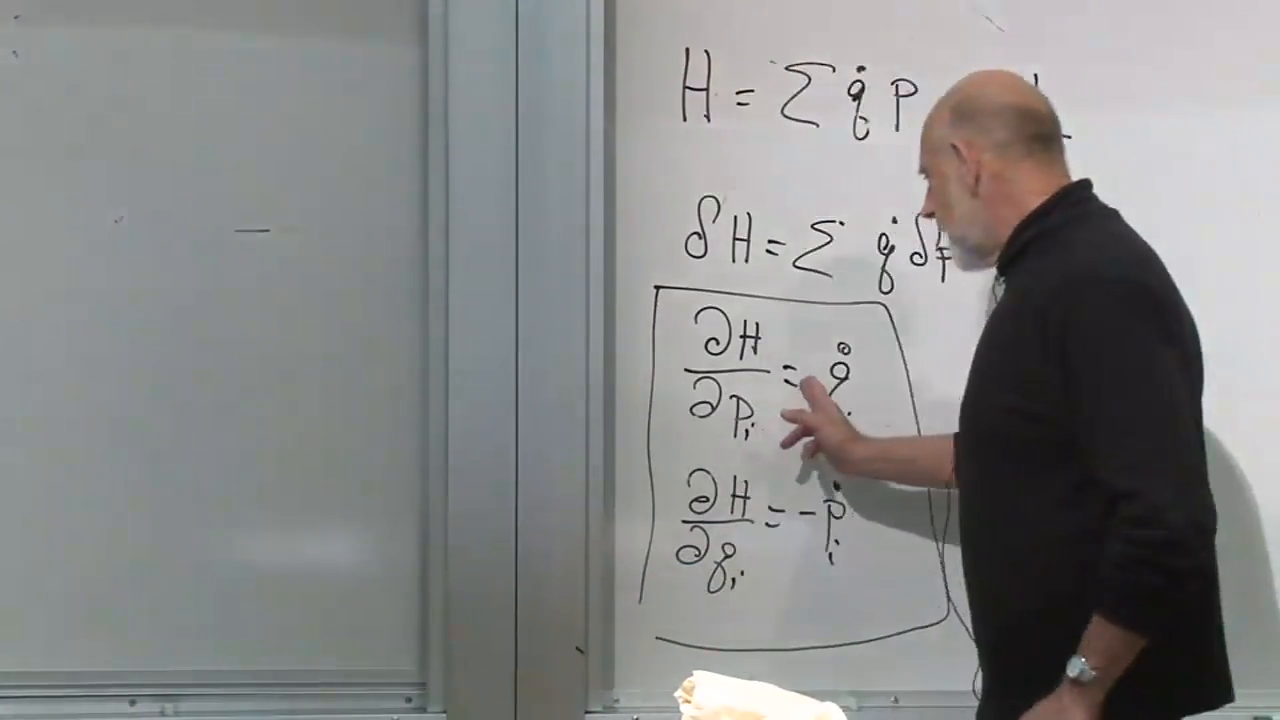
\includegraphics[width=0.78\textwidth]{lecture_06_figure_03.png}
  \caption{Định nghĩa Hamiltonian, biến phân của nó, và các phương trình chính tắc
  được đóng khung.}
  \lectureframe{01:22:18}
\end{figure}

Với \(n\) tọa độ, đây là \(2n\) phương trình bậc nhất.  Dạng thức
Euler--Lagrange trái lại cung cấp \(n\) phương trình bậc hai.
Lượng dữ liệu ban đầu và nội dung vật lý là như nhau.

\section{Chuyển động dao động tử như một phép quay cứng}

Áp dụng phương trình ~\eqref{eq:l6-hamilton-equations} cho
phương trình ~\eqref{eq:l6-oscillator-hamiltonian} ta được
\begin{equation}
  \dot q=\omega p,
  \qquad
  \dot p=-\omega q.
  \label{eq:l6-oscillator-first-order}
\end{equation}
Lấy đạo hàm phương trình thứ nhất và dùng phương trình thứ hai,
\begin{equation}
  \ddot q=\omega\dot p=-\omega^2q.
  \label{eq:l6-oscillator-second-order}
\end{equation}
Do đó, hai phương trình bậc nhất này chính xác là phương trình dao động tử
bậc hai quen thuộc, cùng với định nghĩa của động lượng.

Trong không gian pha, vectơ vận tốc tại \((q,p)\) là
\((\dot q,\dot p)=(\omega p,-\omega q)\), tiếp tuyến với đường tròn năng lượng.
Mọi bán kính đều quay với cùng tốc độ góc \(\omega\).  Có thể hình dung toàn bộ mặt phẳng
như một chong chóng cứng hoặc như một chất lỏng hư cấu không nén được.
Các điểm của nó tuần hoàn; chúng không bị ép vào một điểm hút cũng không tản ra từ một
nguồn.

\begin{figure}[htbp]
  \centering
  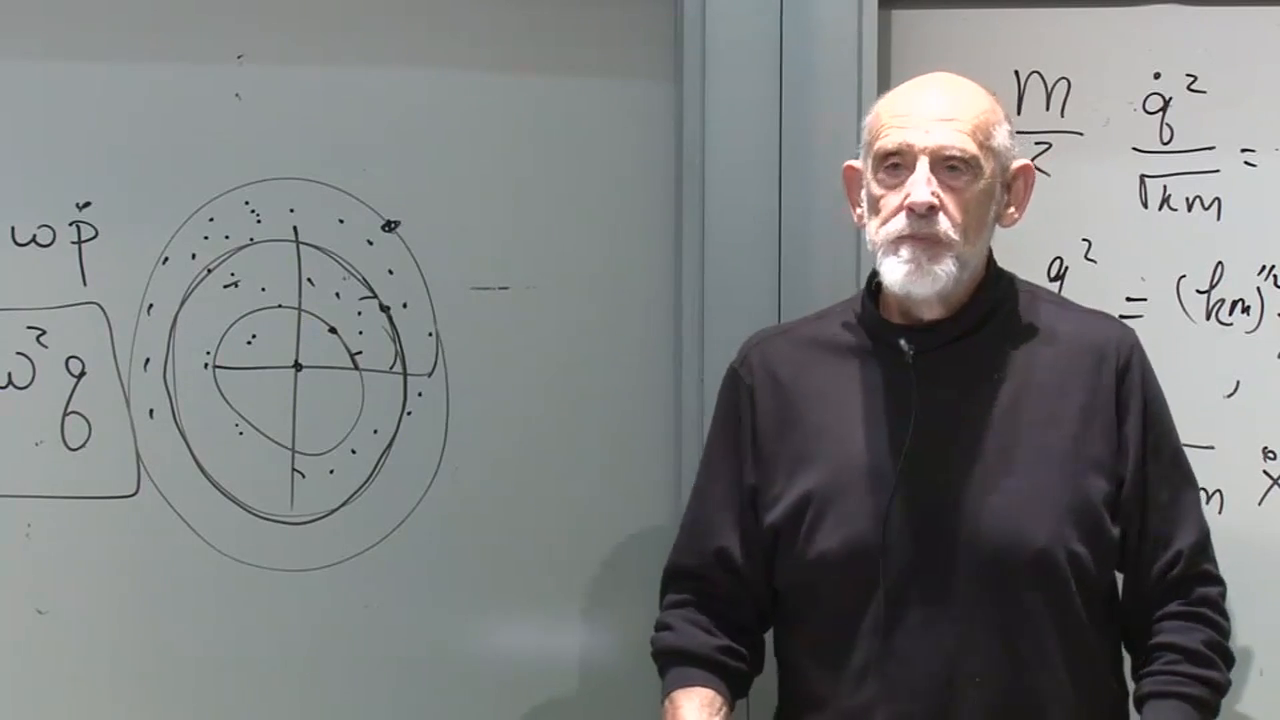
\includegraphics[width=0.86\textwidth]{lecture_06_figure_04.png}
  \caption{Một đám mây các điểm ban đầu phân bố trên các quỹ đạo lồng nhau trong không gian pha.
  Sự tiến hóa Hamilton làm dịch chuyển đám mây ấy thay vì làm nó sụp đổ
  vào một trạng thái ưu tiên.}
  \lectureframe{01:39:27}
\end{figure}

\begin{figure}[htbp]
  \centering
  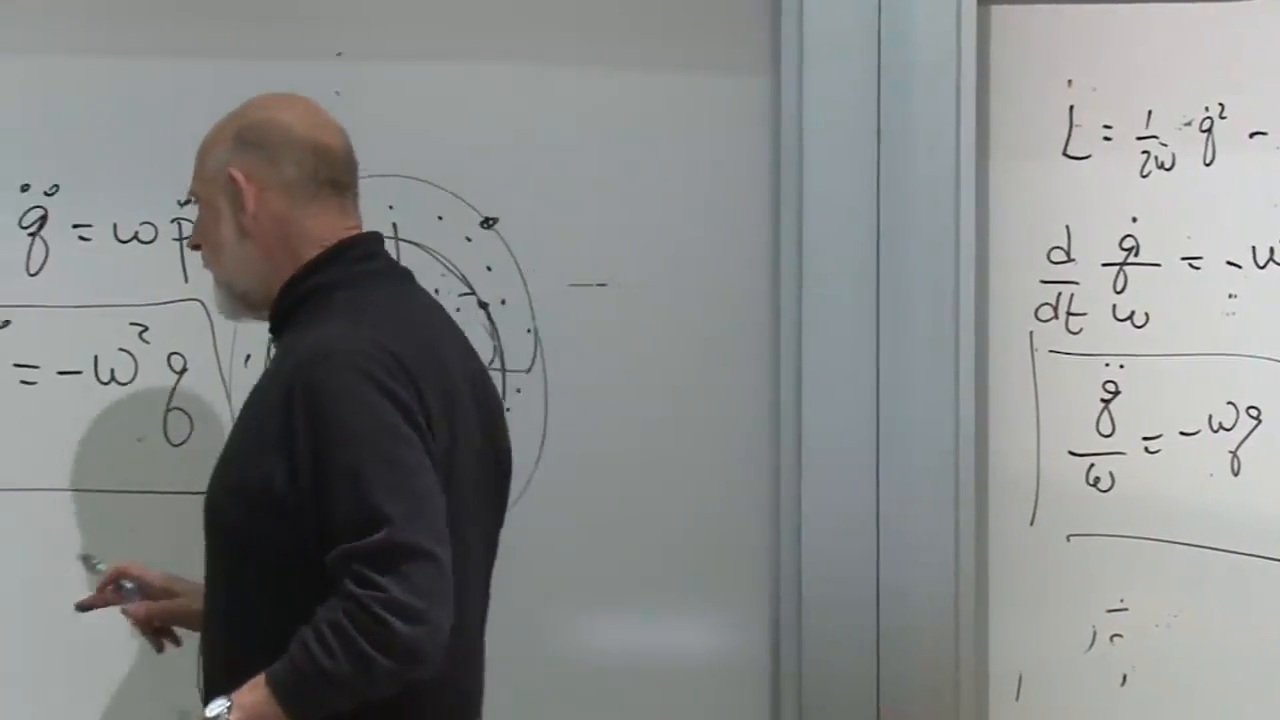
\includegraphics[width=0.90\textwidth]{lecture_06_figure_05.png}
  \caption{Đồ hình pha của dao động tử bên cạnh phương trình
  Euler--Lagrange tương đương
  \(\ddot q/\omega=-\omega q\).}
  \lectureframe{01:42:10}
\end{figure}

Bước tiếp theo sẽ là biến phép tương tự chất lỏng thành một định lý: dòng Hamilton
không có hội tụ hay phân kỳ cục bộ.  Kết quả đó nối lại cơ học liên tục
với các ánh xạ trạng thái khả nghịch đã được xét ở đầu khóa học.

\section{Những câu hỏi làm lộ rõ sự lựa chọn tọa độ}

\begin{classroomqa}
  \audiencequestion{Giả thiết rằng có thể giải các vận tốc theo
  \(q\) và \(p\) là một định lý hay một tính chất thực nghiệm của các hệ vật lý?
  \lecturetimestamp{01:29:08--01:29:45}}
  \lecturerresponse{Trong cách phát triển sơ cấp này, đó là một quy luật
  thực nghiệm, với một động cơ sâu xa hơn đến từ cơ học lượng tử.  Nói
  chính xác hơn, phương trình ~\eqref{eq:l6-legendre-map} phải có Jacobian không suy biến
  theo các vận tốc.  Cơ học hiện đại cũng chứa các Lagrangian suy biến quan trọng,
  đặc biệt là các hệ có ràng buộc và các hệ chuẩn, nhưng dạng thức
  Hamilton của chúng cần thêm công cụ ràng buộc.}
\end{classroomqa}

Một thắc mắc về thứ nguyên giải thích vì sao dao động tử được viết dưới
dạng không quen thuộc của phương trình ~\eqref{eq:l6-rescaled-lagrangian}.  Thay vào đó, hãy bắt đầu với
tọa độ thông thường \(x\):
\begin{equation}
  L=\frac{m}{2}\dot x^2-\frac{k}{2}x^2,
  \qquad
  \omega=\sqrt{\frac{k}{m}}.
  \label{eq:l6-ordinary-oscillator}
\end{equation}
Chọn
\begin{equation}
  q=(km)^{1/4}x.
  \label{eq:l6-oscillator-rescaling}
\end{equation}
Khi đó \(q^2=\sqrt{km}\,x^2\) và
\(\dot q^2=\sqrt{km}\,\dot x^2\), biến đổi
phương trình ~\eqref{eq:l6-ordinary-oscillator} chính xác thành
phương trình ~\eqref{eq:l6-rescaled-lagrangian}.  \(q\) mới là một tọa độ suy rộng đã được thích nghi,
không phải một độ dài, và liên hợp của nó \(p\) không phải là động lượng
cơ học thông thường \(p_x=m\dot x\).

\begin{figure}[htbp]
  \centering
  \includegraphics[width=0.86\textwidth]{lecture_06_figure_15.png}
  \caption{Phép đổi tỉ lệ theo thứ nguyên từ tọa độ dao động tử thông thường
  \(x\) sang tọa độ đã được thích nghi \(q=(km)^{1/4}x\).}
  \lectureframe{01:36:10}
\end{figure}

\begin{classroomqa}
  \audiencequestion{Làm sao \(\omega p=\dot q\) có thể nhất quán về thứ nguyên,
  và vì sao lại chọn các biến này?
  \lecturetimestamp{01:29:46--01:39:22}}
  \lecturerresponse{Ký hiệu \(q\) không bắt buộc phải có thứ nguyên của
  độ dài, và liên hợp của nó \(p\) không bắt buộc phải có thứ nguyên của
  \(m\dot x\).  Phép đổi tỉ lệ trong phương trình ~\eqref{eq:l6-oscillator-rescaling}
  bảo toàn thứ nguyên của Lagrangian và làm cho \(q\) và \(p\) xuất hiện
  đối xứng trong \(H\).  Trong các biến ban đầu,
  \[
    H=\frac{p_x^2}{2m}+\frac{kx^2}{2},
  \]
  nên các đường đồng năng lượng trong mặt phẳng \((x,p_x)\) là các elip.  Trong
  mặt phẳng đã được thích nghi \((q,p)\), chúng là các đường tròn.  Phép đổi tỉ lệ được chọn để làm
  hiện rõ tính đối xứng ấy.}
\end{classroomqa}

\begin{classroomqa}
  \audiencequestion{Làm sao \(2n\) phương trình Hamilton bậc nhất có thể
  tương đương với \(n\) phương trình Lagrange bậc hai?
  \lecturetimestamp{01:39:24--01:42:30}}
  \lecturerresponse{Đối với dao động tử, lấy đạo hàm
  \(\dot q=\omega p\) và thế \(\dot p=-\omega q\); cặp phương trình trở thành
  \(\ddot q=-\omega^2q\).  Nếu xuất phát trực tiếp từ Lagrangian, ta được
  \[
    \frac{d}{dt}\left(\frac{\dot q}{\omega}\right)
      =-\omega q,
  \]
  đó là cùng một phương trình bậc hai.  Có thể xem một phương trình Hamilton
  là định nghĩa xung lượng từ vận tốc, còn phương trình kia cho sự tiến hóa của
  xung lượng ấy.}
\end{classroomqa}

\section{Vì sao không gian pha và thế năng lại quan trọng}

\begin{classroomqa}
  \audiencequestion{Sức mạnh của Hamiltonian có hàm ý rằng không gian pha
  là một biểu diễn hình học tốt hơn không gian cấu hình không?
  \lecturetimestamp{01:42:33--01:44:38}}
  \lecturerresponse{Chúng phục vụ những mục đích khác nhau.  Không gian pha làm cho các chu trình,
  các mặt đồng năng lượng, và sự vắng mặt của hội tụ hay phân kỳ
  trở nên đặc biệt minh bạch.  Không gian cấu hình có thể thích hợp hơn cho những
  câu hỏi khác.  Lý do sâu xa hơn để nhấn mạnh \(H\) là nó trở thành một
  đối tượng trung tâm và trực quan hơn trong cơ học lượng tử, một trong những chủ đề hiện đại mà phần cơ học này hướng tới.}
\end{classroomqa}

\begin{classroomqa}
  \audiencequestion{Có nên xem thế năng là tích phân của
  lực không?
  \lecturetimestamp{01:44:40--01:45:45}}
  \lecturerresponse{Đối với các lực bảo toàn, phát biểu đó là đúng, sai khác một
  hằng số và với dấu thích hợp.  Chiều ngược lại hữu ích hơn là
  xem thế năng là đại lượng cơ bản và suy ra lực suy rộng từ nó:
  \[
    F_i=-\frac{\partial V}{\partial q_i}.
  \]
  Đó chính là hạng xuất hiện trong
  \(\dot p_i=\partial L/\partial q_i\) khi \(L=T-V\) và động năng
  không phụ thuộc tường minh vào \(q_i\).}
\end{classroomqa}

\begin{classroomqa}
  \audiencequestion{Con đường này hướng tới vật lý hiện đại nhằm
  soi sáng những bài toán tuyến đầu nào?
  \lecturetimestamp{01:45:46--01:47:47}}
  \lecturerresponse{Con đường này dẫn tới hấp dẫn lượng tử và vũ trụ học;
  vật lý hạt cơ bản, bao gồm khu vực Higgs và neutrino;
  thuyết tương đối; lý thuyết dây; và lý thuyết trường lượng tử.  Bài toán
  lý thuyết dai dẳng là ghép những mảnh này vào một cấu trúc nhất quán duy nhất,
  đặc biệt là cơ học lượng tử với hấp dẫn và vũ trụ học với vật lý
  hạt.  Đây là một mô tả về tuyến đầu như nó hiện ra vào 2011, chứ không phải một
  khẳng định rằng lời giải của nó đã được biết.}
\end{classroomqa}

Hai ví dụ có ràng buộc và dao động tử giờ đây khớp vào cùng một bức tranh.
Tọa độ suy rộng loại bỏ những lực không cần thiết.  Đối xứng chọn ra các
xung lượng chính tắc được bảo toàn.  Biến đổi Legendre thay các vận tốc bằng
các xung lượng, và các phương trình Hamilton biến động lực học thành một dòng trên không gian pha.
Với dao động tử, dòng ấy là một phép quay cứng; với một hệ tổng quát, hình học của nó sẽ cung cấp ý nghĩa liên tục chính xác của chuyển động khả nghịch.
